\section{Progettazione}

\subsection{Use-Case Diagram}
Per ciascuna tipologia di utente (ospite, cliente, ristoratore) sono stati individuati 
i casi d'uso principali, dalla ricerca di ristoranti alla gestione 
di recensioni e risposte.
\'E stato redatto uno Use-Case Diagram che rappresentasse le 
principali interazioni tra gli utenti e il sistema.
\begin{figure}[H]
  \centering
  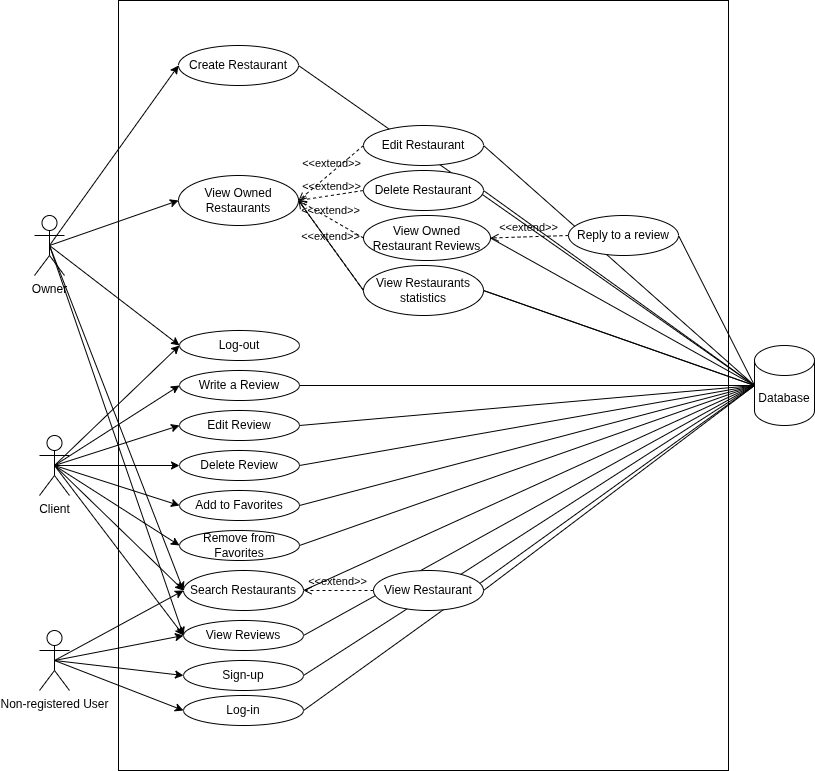
\includegraphics[width=\textwidth]{images/UML-Use-Case.png}
  \caption{User-Case Diagram}
  \label{fig:use-case-diagram}
\end{figure}
Basandosi sul diagramma si è poi proceduto ad articolare le 
singole funzionalità in modo da poterle implementare
in maniera modulare attraverso la Progettazione Orientata agli Oggetti.

\subsection{Class Diagram}
Al fine di rappresentare le classi e le loro relazioni, dallo 
Use-Case Diagram è stato sviluppato un Class Diagram che potesse 
racchiudere le classi principali del sistema.
\begin{figure}[H]
  \centering
  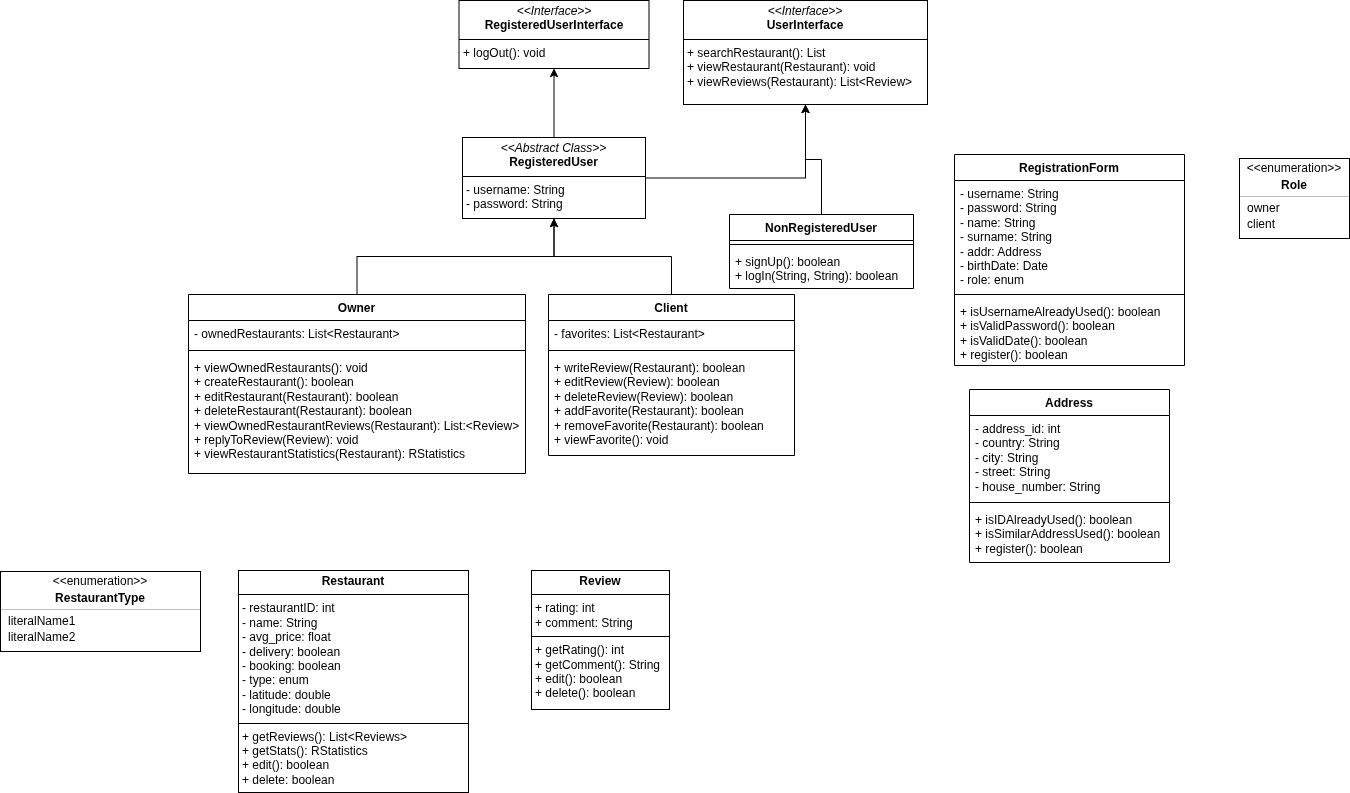
\includegraphics[width=\textwidth]{images/UML-Class-Diagram.png}
  \caption{Class Diagram}
  \label{fig:class-diagram}
\end{figure}
Il diagramma è stato poi utilizzato per implementare le classi 
in Java, seguendo le relazioni e le associazioni
indicate.\\
In particolare le classi e i metodi principali sono stati inseriti 
nel modulo \textit{common} e utilizzati come base fondante del progetto 
per una corretta interazione tra client e server.

\subsection{Architettura del Sistema}
Il sistema è basato su un'architettura Client-Server.\\
Si è scelto di utilizzare Java RMI per la comunicazione tra client e server,
in modo da poter sfruttare le funzionalità di Remote Method Invocation 
e garantire una comunicazione semplice ed efficace.
Il server espone i servizi attraverso un Registry RMI sulla porta 
\texttt{1099}, permettendo ai client di accedere ai metodi remoti.
Il client, a sua volta, si connette al server per invocare i metodi
e ricevere le risposte.\\

\'E stato fondamentale definire delle interfacce comuni a Client 
e Server, in modo da garantire una comunicazione coerente e
facilitare l'implementazione delle funzionalità.
Per questa ragione il progetto è suddiviso in tre moduli principali:
\begin{itemize}
  \item \textbf{client}: implementa il client e la sua interfaccia grafica
  \item \textbf{common}: contiene le classi e le interfacce comuni per il trasferimento dei dati tra client e server
  \item \textbf{server}: implementa il server e gestisce la connession con il database
\end{itemize}

\subsection{Flusso delle Informazioni}
Nel modulo \textit{common} sono definite le interfacce comuni e le 
classi serializzabili definite con il pattern 
Data Transfer Object (DTO), che permettono di trasferire
i dati tra client e server in modo strutturato.\\
Il trasferimento di informazione avviene attraverso le interfacce 
definite nel package \textit{common} implementate nel server e 
accessibili al client tramite il Registry.
I DTO serializzabili possono essere passati come argomento ai 
metodi invocati.
L'elaborazione viene presa 
in carico dagli oggetti Data Access Object (DAO) 
presenti sul server che
gestiscono l'interazione con il database.\\
Il server, una volta ricevuti i dati, li elabora e restituisce
le risposte al client, che le visualizza nell'interfaccia grafica.\\
Questa architettura consente di mantenere una chiara separazione
tra le responsabilità del client e del server, facilitando la
manutenzione e la semplicità del sistema.

\begin{figure}[H]
  \centering
  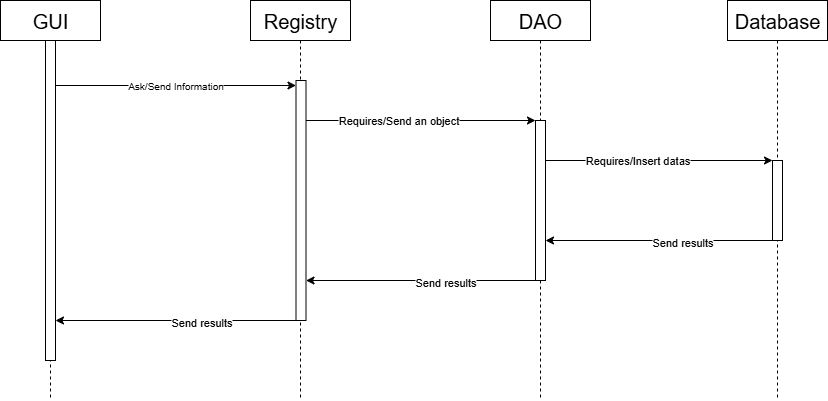
\includegraphics[width=\textwidth]{images/UML-interaction.png}
  \caption{Interaction Diagram}
  \label{fig:interaction-diagram}
\end{figure}
